\documentclass{article}
\usepackage{amsmath}
\usepackage{amssymb}
\usepackage{tikz}
\usepackage{tikz}
\usetikzlibrary{positioning,shapes,arrows,automata,decorations.pathreplacing,angles,quotes}

\begin{document}

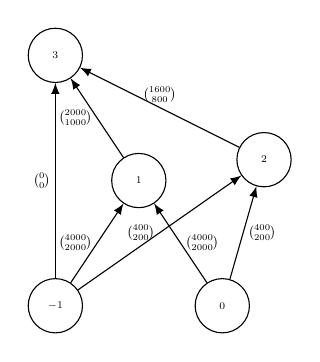
\begin{tikzpicture}[scale=.53, transform shape]
\begin{pgfscope}
  \tikzstyle{every node}=[draw,circle,minimum size=1.3cm]
  \node (-1) at (0,0) {\scriptsize $-1$};
  \node (0) at (4,0) {\scriptsize $0$};
  \node (1) at (2,3) {\scriptsize $1$};
  \node (2) at (5,3.5) {\scriptsize $2$};
  \node (3) at (0,6) {\scriptsize $3$};
\end{pgfscope}
\begin{scope}[-latex]
 \draw (-1) -- (1) node[midway,left] {\footnotesize $\binom{4000}{2000}$};
 \draw (0) -- (1) node[midway,right] {\footnotesize $\binom{4000}{2000}$};
 \draw (-1) -- (2) node[midway,left] {\footnotesize $\binom{400}{200}$};
 \draw (0) -- (2) node[midway,right] {\footnotesize $\binom{400}{200}$};
 \draw (-1) -- (3) node[midway,left] {\footnotesize $\binom{0}{0}$};
 \draw (1) -- (3) node[midway,left] {\footnotesize $\binom{2000}{1000}$};
 \draw (2) -- (3) node[midway,above] {\footnotesize $\binom{1600}{800}$};
\end{scope}
\end{tikzpicture}

\end{document}